\chapter{Introdução}



\chapter{Apresentação das equações utilizadas}

\section{Filtração}


Para uma filtração sólido-líquido com formação de torta e considerando a torta como um meio poroso, aplica-se a equação do movimento para a torta:

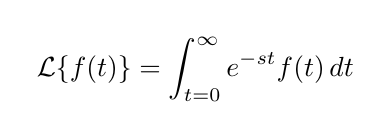
\begin{tikzpicture}
\draw (0,0) node{$\displaystyle{
		\mathcal{L} \lbrace f(t)\rbrace = \int_{t=0}^\infty e^{-st} f(t)\,dt}$};
\end{tikzpicture}

\begin{equation}\label{key}
\rho\left[\varepsilon \frac{\partial \frac{q}{\varepsilon}}{\partial t}+\nabla\left(\frac{q}{\varepsilon}\right) q\right]=-\nabla P+\nabla \tau-m+\rho g
\end{equation}


onde:

\begin{itemize}

\item $\rho$ = densidade
\item $\varepsilon$ = porosidade da torta
\item q = velocidade superficial
\item P = pressão do sistema
\item $\tau$ = parâmetro proveniente de forças viscosas
\item g = aceleração da gravidade
\item m = massa de sólidos na torta

\end{itemize}

Suposições:

\begin{itemize}
\item Sem forças de campo;
\item Estado estacionário;
\item $\mathrm{\nabla\tau}= 0$ (sem interação viscosa);
\item Meio poroso isotrópico (k = cte.);
\item Escoamento a baixas velocidades ($Re_{MP}<1,0$)
\item Fluído;
\item Meio poroso rígido ($\varepsilon$ = cte.);
\item Meio poroso estacionário;
\item Escoamento isotérmico e incompressível ($\rho$=cte.);
\item Unidimensional e horizontal.
\end{itemize}

Então:

\begin{equation}\label{key}
\mathrm{m}=-\nabla P
\end{equation}

Com equação do movimento e a de  Darcy:

\begin{equation}\label{key}
\frac{d P}{d x}=\frac{\mu}{k} q
\end{equation}


E utilizando a definição de porosidade:

\begin{equation}\label{key}
\mathrm{dM}=\rho_{s}(1-\varepsilon) A d x
\end{equation}

Onde:

\begin{itemize}
\item $\mu$ = viscosidade do fluido;
\item A = área de filtração;
\item $\rho_{s}$ = densidade do sólido.
\end{itemize}

Fazendo as devidas substituições: e considerando PL = constante:

\begin{equation}\label{key}
d(P L-P)=\left(\frac{\mu q}{k \rho_{s}(1-\varepsilon) A}\right) d M
\end{equation}

A resistividade da torta ($\alpha$):

\begin{equation}\label{key}
\alpha=\frac{1}{k \rho_{s}(1-\varepsilon)}
\end{equation}

Logo,

\begin{equation}\label{key}
\mathrm{d}(\mathrm{PL}-\mathrm{P})=\left(\frac{\mu q a}{A}\right) d M
\end{equation}


\section{Dimensionamento Industrial}


Para o escalonamento de um filtro piloto para um filtro industrial consideramos que ambos operam com a mesma suspensão, a mesma queda de pressão e sob a mesma temperatura. Utilizando o subscrito ‘P’ para Piloto e ‘I’ para Industrial, temos as Equações \ref{DI1} e \ref{DI2} :

\begin{equation}\label{DI1}
V_{t P}=\frac{A_{P}}{2} e_{P}
\end{equation}

\begin{equation}\label{DI2}
V_{t I}=\frac{A_{I}}{2} e_{I}
\end{equation}


Em que, Vt é o volume da torta e  “e” a espessura do quadro. Considerando que o volume de torta é proporcional ao volume de filtrado (V) e combinando \ref{DI1}, \ref{DI2} à equação de trabalho, temos as Equações \ref{DI3} e \ref{DI4} :

\begin{equation}\label{DI3}
\frac{t_{P}}{t_{I}}=\frac{\left(\frac{V_{P}}{A_{P}}\right)^{2}}{\left(\frac{V_{I}}{A_{I}}\right)^{2}}
\end{equation}

\begin{equation}\label{DI4}
t_{I}=t_{P}\left(\frac{e_{I}}{e_{P}}\right)^{2}
\end{equation}


Com o tempo total de filtração na escala piloto, obtém-se o tempo total de filtração na escala industrial pela equação 13. Sabendo que o volume de filtrado industrial pode ser determinado pela Equação \ref{DI5}, da Equação \ref{DI3} calcula-se a área total de filtração industrial.

\begin{equation}\label{DI5}
V_{I}=P_{t} \cdot T_{I}
\end{equation}

Em que P é a vazão de produção da unidade industrial.
A vazão de produção de filtrado pode ser calculada como sendo a razão entre o volume de filtrado e o tempo total do ciclo de operação, incluindo o tempo de filtração , o tempo de lavagem dos quadros  e o tempo de montagem dos quadros  para a próxima operação, de acordo com a Equação \ref{DI6}. 

\begin{equation}\label{DI6}
P=\frac{V}{t_{f i l t}+t_{l a v}+t_{m o n t}}
\end{equation}


\chapter{Materiais e Métodos}

\section{Materiais}

\begin{itemize}

\item Suspensão de carbonato de cálcio;
\item Três vidros de relógio numerados;
\item Três becher numerados;
\item Duas provetas graduadas de 2L;
\item Um bastão de vidro;
\item Cronômetro (foi utilizado o cronômetro do celular de um dos integrantes do grupo);
\item Régua;
\item Espátula;
\item Filtro prensa (formado por dois quadros sem recheio, três placas rugosas e dois meios filtrantes);
\item Balança digital;
\item Estufa.


\end{itemize}

\section{Métodos}

Os bécher e vidros de relógio foram pesados e enumerados. Foram medidas as dimensões do quadro do filtro prensa com o auxilio de uma régua. 

O filtro prensa foi montado utilizando dois meios filtrantes. Estes foram umedecidos previamente para minimizar vazamentos. O filtro prensa utiliza dois quadros vazados que servem de suporte para os meios filtrantes e três placas rugosas. Durante a montagem do filtro prensa é realizada sobre o trilho do equipamento com placas e quadros intercalados de forme que duas placas fiquem nas extremidades. Foi verificada sistematicamente com uso de uma caneta se os furos de placas e quadros coincidem para que a suspensão possa para por todo o circuito do filtro-prensa. Após a verificação do ajuste do filtro, apertou-se o parafuso que mantem os quadros unidos e vedados contra o vazamento.

A solução de carbonato de cálcio presente no tanque de alimentação foi homogeneizada com auxílio de um bastão de vidro. \emph{Três amostras foram retiradas da suspensão} e pesadas nos bécher previamente pesados e identificados. Essa amostras foram então encaminhadas para uma estufa \emph{desligada durante cinco dias. No quinto dia a estufa foi ligada e. no sexto dia, as amostras secas foram pesadas novamente.}
 
Antes do início da filtração as provetas foram posicionadas de forma a coletar a solução filtrada e facilitar a troca rápida quando a primeira proveta chegar ao nível máximo. Com o tanque de alimentação já em recirculação, foi aberta a válvula a montante do filtro-prensa.

Com auxilo de provetas, o filtrado foi coletado. Durante este processo foram realizadas a marcação de volume filtrado em relação ao tempo de filtração. Para a marcação do tempo foi utilizado cronometro de celular operado por um dos alunos e com avisos sonoros dos alunos que operavam a coleta do filtrado na proveta.

A vazão de filtrado diminuiu durante a filtração e o experimento foi finalizado quando esta vazão ficou próxima de nula com a saída de gotas de filtrado. Foi coletado um total de 3,7 L de filtrado. A pressão de operação foi anotada e se manteve constante.


A torta formada nos quadros foi retirada e colocada sobre uma placa. Foram retiradas três alíquotas e alocadas em vidros de relógio já pesados e identificados. As amostras recolhidas nos vidros de relógio foram pesadas e mantidas na estufa desligada durante cinco dias. No quinto dia a estufa foi ligada e, no sexto dia, as amostras secas foram pesadas.

Ao final da prática, o filtrado e as tortas foram devolvidos ao tanque de alimentação.



\chapter{Resultados e Discussão}

\section{Propriedades Físicas}

Os dados apresentados na tabela a seguir foram obtidas do Manual de Engenharia Química, Perry and Chilton, 8a edição.

\begin{table}[H]
	\centering
	\begin{tabular}{|c|c|}
		\hline
		\rowcolor[HTML]{DAE8FC} 
		\textbf{Propriedade} & \textbf{Valor} \\ \hline
		Densidade da Água ($\rho F$) & $1,000 g \ \cdot cm^{-3}$ \\ \hline
		Viscosidade da Água ($\mu F$) & $1,00 \cdot E-3 \ Pa.s$ \\ \hline
		Densidade do Sólido ($\rho S$) & $2,711 \ g \cdot cm^{-3}$ \\ \hline
	\end{tabular}
	\caption{Propriedades Físicas da água e do sólido.}
	\label{tab:prop}
\end{table}


\section{Dados Experimentais}

\subsection{Cálculo da concentração em suspensão.}

A partir das massas da Tabela \ref{tab:massas}, calculou-se a concentração da suspensão da seguinte forma:

\begin{itemize}
	\item Massa da suspensão = (bécher + suspensão) - (bécher vazio)
	\item Massa seca = (bécher + massa seca) - (bécher vazio) 
	\item Concentração =  $\dfrac{\text{Massa de }CaCO_{3}}{\text{Massa da Suspensão}} $
\end{itemize}



\begin{table}[H]
	\centering
	\begin{tabular}{|c|c|c|c|}
		\hline
		\rowcolor[HTML]{DAE8FC} 
		\textbf{Bécher} & \textbf{Bécher vazio (g)} & \textbf{Bécher + suspensão (g)} & \textbf{Bécher  + sólido seco (g)} \\ \hline
		1 & 40,494 & 75,736 & 451,748 \\ \hline
		2 & 298,228 & 589,628 & 336,909 \\ \hline
		3 & 300,684 & 580,403 & 337,752 \\ \hline
	\end{tabular}
	\caption{Massas obtidas para o cálculo da concentração média da suspensão a ser filtrada.}
	\label{tab:massas}
\end{table}


As massas de sólido e de água foram calculadas para cada uma das três amostras e as concentrações obtidas estão apresentadas a seguir:

\begin{table}[H]
	\centering
	\begin{tabular}{|c|c|c|c|}
		\hline
		\rowcolor[HTML]{DAE8FC} 
		\textbf{Amostra} & \textbf{Massa de $CaCO_{3}$ (g)} & \textbf{Massa  da Suspensão (g)} & \textbf{Concentração $\frac{g CaCO_{3}}{g susp.}$} \\ \hline
		1 & 46,808 & 35,242 & 0,13282 \\ \hline
		2 & 38,681 & 29,14 & 0,13274 \\ \hline
		3 & 37,068 & 279,719 & 0,13252 \\ \hline
		\multicolumn{3}{|c|}{Média} & 0,13269 \\ \hline
	\end{tabular}
	\caption{Massas utilizadas no cálculo da concentração média da suspensão a ser filtrada.}
	\label{tab:massas2}
\end{table}

A concentração média obtida foi de 0,13269 $\dfrac{g \text{ de }  CaCO_{3}}{g \text{ de } susp.}$.


\subsection{Cálculo da porosidade média da torta}

\begin{table}[H]
	\centering
	\fontsize{10px}{10}\selectfont
	\begin{tabular}{|c|c|c|c|c|c|}
		\hline
		\rowcolor[HTML]{DAE8FC} 
		\textbf{\begin{tabular}[c]{@{}c@{}}Vidro de\\ Relógio\end{tabular}} & \textbf{\begin{tabular}[c]{@{}c@{}}Vidro de \\ Relógio vazio \\ (g)\end{tabular}} & \textbf{\begin{tabular}[c]{@{}c@{}}Vidro  de Relógio \\ + torta úmida\\ (g)\end{tabular}} & \textbf{\begin{tabular}[c]{@{}c@{}}Vidro de Relógio \\ + torta seca\\ (g)\end{tabular}} & \textbf{\begin{tabular}[c]{@{}c@{}}Torta Úmida\\ (g)\end{tabular}} & \textbf{\begin{tabular}[c]{@{}c@{}}Torta Seca \\ (g)\end{tabular}} \\ \hline
		1 & 343,432 & 514,536 & 449,302 & 171,104 & 105,870 \\ \hline
		2 & 44,149 & 594,163 & 529,781 & 152,673 & 88,291 \\ \hline
		3 & 367,894 & 532,342 & 462,667 & 164,448 & 94,773 \\ \hline
	\end{tabular}
	\caption{Massas dos vidros de relógio e tortas (g) obtidas para o cálculo da porosidade média da torta.}
	\label{tab:massas3}
\end{table}


Obtém-se o volume da água pela equação a seguir:

\begin{equation}\label{key}
V_{\text{água}} = \dfrac{M_{\text{água}}}{\rho_{\text{água}}}=\dfrac{M_{torta} - M_{\text{torta seca}}}{\rho_{\text{água}}}
\end{equation}

E o volume de torta seca:

\begin{equation}\label{key}
V_{\text { torta seca }}=\frac{M_{\text {torta seca}}}{\rho _{C a C O_{3}}}
\end{equation}

Por fim, obtém-se o Volume total por meio de:

\begin{equation}\label{key}
V_{total} = V_{\text{torta seca}}+V_{\texttt{água}} = M_{\texttt{torta seca}} + \dfrac{M_{torta} - M_{\texttt{torta seca}}}{\rho_{\text{água}}}
\end{equation}


Os resultados obtidos através dos cálculos demonstrados estão apresentados na Tabela \ref{tab:massas4}.


\begin{table}[H]
	\centering
		\begin{tabular}{|c|c|c|c|}
			\hline
			\rowcolor[HTML]{DAE8FC}
			\textbf{Amostra} & \textbf{\begin{tabular}[c]{@{}c@{}}Água\\ $(cm^{3})$ \end{tabular}} & \textbf{\begin{tabular}[c]{@{}c@{}}Torta seca\\ $(cm^{3})$ \end{tabular}} & \textbf{\begin{tabular}[c]{@{}c@{}}Torta Úmida \\ $(\text{Volume total - }cm^{3})$ \end{tabular}} \\ \hline
			1 & 6,5234 & 3,9052 & 10,4286 \\ \hline
			2 & 6,4382 & 3,2568 & 9,69497 \\ \hline
			3 & 6,9675 & 3,4959 & 10,46337 \\ \hline
	\end{tabular}
	\caption{Massas da torta úmida e seca.}
	\label{tab:massas4}
\end{table}




Por meio da Equação \ref{poro} foi possível determinar a porosidade média da torta:

\begin{equation}\label{poro}
\varepsilon = \dfrac{V_{\text{água}}}{V_{total}} = 1 - \dfrac{V_{\text{torta seca}}}{V_{total}}
\end{equation}

\begin{table}[H]
	\centering
	\begin{tabular}{|c|c|}
		\hline
		\rowcolor[HTML]{DAE8FC} 
		\textbf{Amostra} & \textbf{\begin{tabular}[c]{@{}c@{}}Porosidade\\   ($\varepsilon$)\end{tabular}} \\ \hline
		1 & 0,6255 \\ \hline
		2 & 0,6641 \\ \hline
		3 & 0,6659 \\ \hline
		Média & 0,6518 \\ \hline
	\end{tabular}
	\caption{Porosidade calculada para cada amostra e porosidade média.}
	\label{tab:poros}
\end{table}


Portanto, a porosidade média da torta é 0,6518.

\subsection{Cálculo da Resistividade da Torta ($\alpha$) e Resistência do Meio Filtrante ($R_m$)}

A resistividade da torta e a resistência do meio filtrante podem ser obtidos por meio do método gráfico no qual plota-se a curva t/V vs V a partir dos dados experimentais da filtração, apresentados na Tabela \ref{tab:corrida}.


\begin{table}[H]
	\centering
	\begin{tabular}{|c|c|c|}
		\hline
		\rowcolor[HTML]{DAE8FC} 
		\textbf{\begin{tabular}[c]{@{}c@{}}tempo \\ (s)\end{tabular}} & \textbf{\begin{tabular}[c]{@{}c@{}}Volume\\   Filtrado \\ (L)\end{tabular}} & \textbf{\begin{tabular}[c]{@{}c@{}}Tempo/Volume\\ (s/L)\end{tabular}} \\ \hline
		3,73 & 0,5 & 7,46 \\ \hline
		10,02 & 1 & 10,02 \\ \hline
		17,45 & 1,5 & 11,63 \\ \hline
		31,25 & 2 & 15,63 \\ \hline
		39,5 & 2,2 & 17,95 \\ \hline
		45,39 & 2,4 & 18,91 \\ \hline
		52,07 & 2,6 & 20,03 \\ \hline
		59,47 & 2,8 & 21,24 \\ \hline
		66,23 & 3 & 22,08 \\ \hline
		74,47 & 3,2 & 23,27 \\ \hline
		90,35 & 3,4 & 26,57 \\ \hline
		106,17 & 3,6 & 29,49 \\ \hline
		120,59 & 3,7 & 32,59 \\ \hline
	\end{tabular}
	\caption{Volume do filtrado (L) em função do tempo (s).}
	\label{tab:corrida}
\end{table}

Com os dados da tabela 7, plotou-se o gráfico a seguir:

\begin{figure}[H]
	\begin{center}
		\includegraphics[scale=1,trim={0 0 0 0}]{figuras/ladeq/filtra/graph1}
		%\vspace{-20pt}
		\caption{Curva de filtração - t/V (s/L) em função de V(L).}
		\label{apaTeo}
	\end{center}
\end{figure}

Os primeiros pontos não apresenta comportamento linear, pois no início do processo ainda não havia uma resistência significativa do meio filtrante e, por isso, a vazão de filtrado ainda era muito alta, obtendo-se assim, um grande volume de filtrado em um curto espaço de tempo, fazendo que a divisão tempo/volume ficasse muito baixo.

Por outro lado, no final do processo, a configuração exponencial do fim do gráfico indica que a torta estava completamente formada e não havia mais vazão de fluido. 

Diante do que foi dito anteriormente, para estimar os parâmetros de resistividade da torta e a resistência do meio filtrante, deve-se trabalhar apenas com a parte do gráfico que apresente comportamento linear. Sendo assim, os pontos iniciais e finais que fogem da linearidade foram desprezados.

\begin{figure}[H]
	\begin{center}
		\includegraphics[scale=1,trim={0 0 0 0}]{figuras/ladeq/filtra/graph2}
		%\vspace{-20pt}
		\caption{Curva de filtração - parte linear de t/V (s/L) em função de V(L).}
		\label{apaTeo}
	\end{center}
\end{figure}



Por fim, a  Resistividade da Torta $(\alpha)$ e Resistência do Meio Filtrante $(R_m)$, são obtidas por meio dos coeficientes angular e linear da equação obtida, de acordo com a equação a seguir:  


\begin{equation}\label{key}
\frac{t}{V}=\frac{\mu_{F}}{A \Delta p_{m}}\left(\frac{\alpha C p_{F} V}{2 A}+R_{m f}\right)
\end{equation}

Diante disso:

\begin{equation}\label{key}
\frac{t}{V}=5,2763 V+6,2747
\end{equation}

\begin{equation}\label{key}
\frac{\alpha \mu_{F} C p_{F}}{2 A^{2} \Delta p_{m}}=5,2763, \quad \frac{\mu_{F R_{m f}}}{A \Delta p_{m}}=6,2747
\end{equation}

A área de filtração pode ser obtida pela seguinte expressão: $A=2A_{P}2(0,9398)$, onde $A_{P}$ é a área de filtração na planta piloto $(A_{P}=16,2 \times16,3 cm^{2}=264,06 cm^{2} = 0,026406 m^{2}$ e 0,9298 é o fator de correção da placa. Desta forma, tem-se $A = 0,09927 m^{2}$.
O valor da queda de pressão foi mantido constante e igual a: $\Delta P= 5 kgf\cdot cm^{-2} = 49067,7 Pa$.
Em posse de todos os dados necessários para o cálculo da resistividade e resistência, basta isolar o $\alpha$ para encontrar o primeiro e o $R_{m}$ para o segundo:

\begin{equation}\label{key}
\alpha=5,2763 \frac{2 A^{2} \Delta p_{m}}{\mu_{F} C p_{F}}, R_{m f}=6,2747 \frac{A \Delta p_{m}}{\mu_{F}}
\end{equation}

\begin{equation}\label{key}
\alpha=3,8451 \times 10^{4} \ \mathrm{m} . \mathrm{kg}^{-1}, R_{m}=3,056 \times 10^{7} \ \mathrm{m}^{-1}
\end{equation}

\chapter{Dimensionamento Industrial}


\section{Dados}
Visando dimensionar um filtro industrial que atenda os seguintes parâmetros obtidos no procedimento experimental:



\begin{itemize}
\item Tempo de desmantelamento, lavagem e montagem do filtro: 20 minutos ou 1200 s (hipótese do grupo)
\item No roteiro diz para considerar $ t_{1} $ e $ t_{4} $ nulos!!!!!!!!!!!!
\item Tempo de filtração em escala piloto: 120,59 s;
\item Volume de filtrado em escala piloto: 3,7 L;
\item Espessura do quadro em escala piloto: 1,1 cm;
\item Pressão de filtração em escala piloto: $\Delta P= 49067,7 \ Pa$
\item Área de filtração em escala piloto: $ 0,026406 m^{2} $
\end{itemize}




Visando os seguintes parâmetros para a produção industrial:

\begin{itemize}
\item Pressão de filtração: Considerar mesma pressão da escala piloto.
\item Espessura do quadro em escala industrial: 3 cm 
\item Produção em escala industrial: 13000 $ \dfrac{L}{h} $ $ \approx 3,61 \ \dfrac{L}{s} $
\end{itemize}

\section{Determinação do tempo de filtração}


\begin{equation}\label{key}
\mathrm{t}_{\mathrm{IND}}=\mathrm{t}_{\mathrm{PIL}}\left(\frac{e_{I N D}}{e_{P I L}}\right)^{2}
\end{equation}


\begin{equation}\label{key}
t_{\mathrm{IND}}=120,59\left(\frac{3}{1,1}\right)^{2}=896,95\ s= 14,9491\ min \approx 15 \ min
\end{equation}

\section{Determinação do volume de filtrado industrial}




\begin{equation}\label{key}
\mathrm{P}_{\mathrm{IND}}=\frac{\mathrm{V}_{\mathrm{IND}}}{\mathrm{t}_{\mathrm{IND}}+t_{L}+t_{D}}
\end{equation}

\begin{equation}\label{key}
3,61=\frac{V_{I N D}}{896,95+1200}
\end{equation}


\begin{equation}\label{key}
\mathrm{V}_{\mathrm{IND}}=7572,321 \ L 
\end{equation}


\section{Determinação da área efetiva de filtração industrial}




\begin{equation}\label{key}
\mathrm{A}_{\mathrm{IND}}=\mathrm{A}_{\mathrm{PIL}} \frac{\mathrm{V}_{\mathrm{IND}}}{\mathrm{V}_{\mathrm{PIL}}} \frac{\mathrm{e}_{\mathrm{PIL}}}{\mathrm{e}_{\mathrm{IND}}}
\end{equation}

\begin{equation}\label{key}
\mathrm{A}_{\mathrm{IND}}=998,74 \frac{7572,321}{3,7} \cdot \frac{1,1}{3}=19,815 \ m^{2}
\end{equation}


\begin{equation}\label{key}
A_{\mathrm{IND}}=19,815 \ m^{2} \times 10,76 \ \frac{f t^{2}}{m^{2}}=213,213 \ f t^{2}
\end{equation}

A fim de propor um quadro específico para a área calculada, utilizou-se como base as tabelas abaixo:

\begin{figure}[H]
	\begin{center}
		\includegraphics[scale=.6,trim={0 0 0 0}]{figuras/ladeq/filtra/tabquadro1}
		%\vspace{-20pt}
		\caption{Relação da área total de filtração com a dimensão dos quadros.}
		\label{tabqua1}
	\end{center}
\end{figure}



\begin{figure}[H]
	\begin{center}
		\includegraphics[scale=.6,trim={0 0 0 0}]{figuras/ladeq/filtra/tabquadro2}
		%\vspace{-20pt}
		\caption{Relação da dimensão dos quadros com a área efetiva de filtração de cada quadro, para quadros de madeira e de metal.}
		\label{tabqua2}
	\end{center}
\end{figure}

Foi escolhido o prato de dimensão igual a 30 in de metal, foi calculado então o número de pratos utilizados na operação industrial.



\begin{equation}\label{key}
N=\frac{213,213}{10,5}= 20,306 \approx 21 \ \text{quadros}
\end{equation}

\section{Projeto industrial do filtro-prensa}


Portanto, diante dos cálculos apresentados, para uma produção de filtrado de 13000 $ \dfrac{L}{h} $ de uma suspensão de carbonato de cálcio na concentração de $ 0,13269 \ \dfrac{g \ CaCO_{3}}{g \ \text{solução}}$ (PODE-SE COLOCAR EM FUNÇÃO H2O) com quadros de 1,2
in de espessura, o grupo propõe o seguinte projeto: 21 quadros de metal de dimensão 30 in e área total efetiva de 213,213 $ ft^{2} $.



\chapter{Conclusões}
